\section{Analysis of Average Word Length ratios}
\subsection{AWL ranges within collections}
The following chart shows the range of the AWL of suttas within the collections.\\

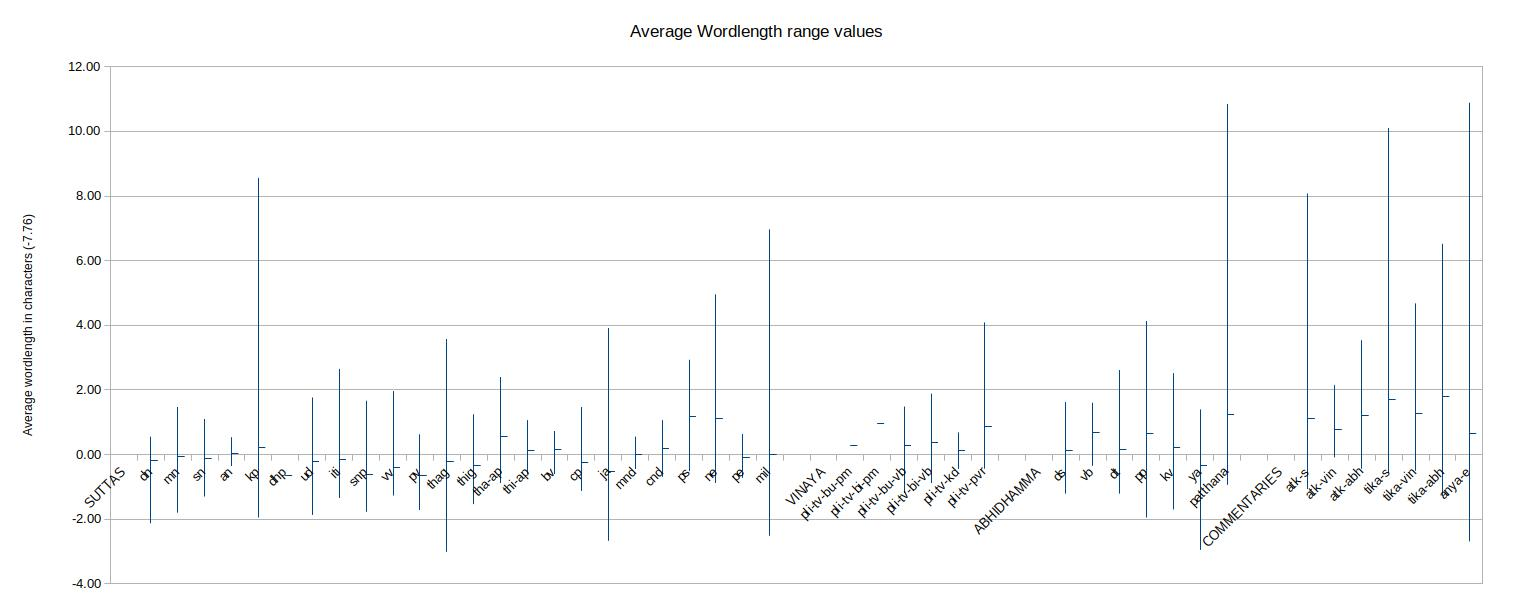
\includegraphics[width=\linewidth]{minmax.jpg}
\captionof{figure}{Variation of the AWL within collections in characters -7.76 (based on mean value of the Aṅguttara Nikāya)}
\label{minmax}

\medskip
The largest variation in the AWL between texts we see in later texts, but the Khuddakapāṭha stands out for it's very high value. This text comprises of eight short texts, which appear to have been collected as a kind of basic study curriculum for novices. The collection itself was probably made in Sri Lanka, but most of the texts are found elsewhere in the nikāyas.

The main reason for the very high-end value of the Khuddakapāṭha we find in only one very well-known word in kp2: "Mālāgandhavilepanadhāraṇamaṇḍanavibhūsanaṭṭhānā". This is a compound that appears in the 10 precepts of the novice. The reason why this word would stand out so much more in this collection as opposed to it's source collections is simply that the text has been taken out of it's original context, which would have been a much longer text so here the word has a much higher impact on the AWL. 

Moreover, although all the suttas in this collection are early, the collection as a whole is not. This can explain the spread in AWL.

Note that for the purposes of this research, the Saṃyutta Nikāya and Aṅguttara Nikāya have been merged into their respective saṃyuttas and nipatas, therewith creating much longer texts which have therefore much more levelled-out values of the AWL. The average AWL will remain the same but the range that is shown will not be representative of the values of the texts therein. A study of the separate texts in each will yield different results.

\subsection{Weighted AWL ratios}
In our analysis of the Jātaka we have seen that the shorter suttas had a relatively larger AWL then the longer ones. A long word in a short sutta will have a much higher impact on the range in the AWL as seen above. To analyse the impact of shorter texts, it is necessary to give a weight value to each, based on their respective length.

We can measure the length of a sutta in two ways, namely by the number of characters or the number of words. The below chart shows the range of the difference between the File Character Weight (FCW) and File Word Weight (FWW)\\

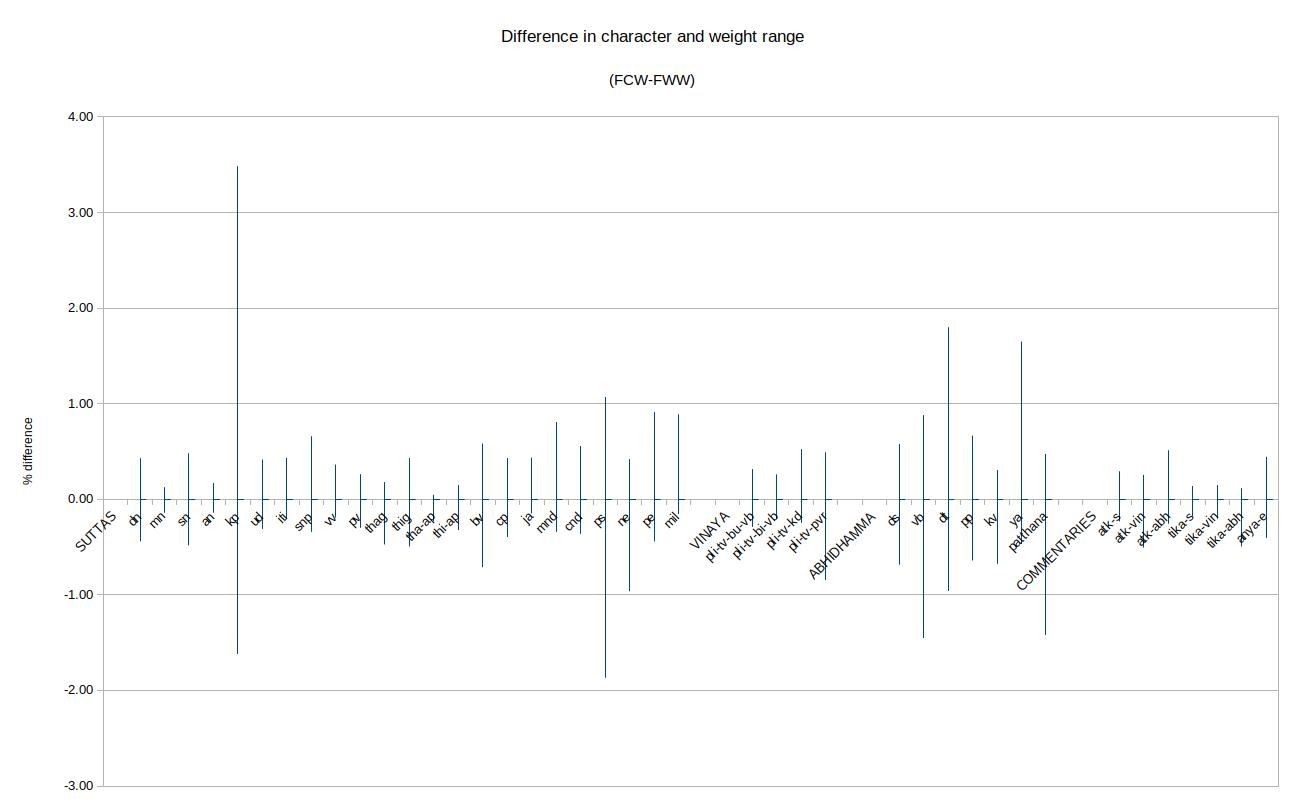
\includegraphics[width=\linewidth]{fcw-fww.jpg}
\captionof{figure}{Range of the difference between the character and word weights per collection}
\label{fcw-fww}

\medskip
What we see here is that collections with a high spread show a large difference between texts as if these texts are of equal length. This means that values higher than 0 have a higher character weight i.e. they contain longer words than average in the collection while the values under 0 represent texts that have more shorter words than average. 

We see in figure \ref{fcw-fww} that the Khuddakapāṭha still shows a very high spread, while the commentaries show a significantly lower spread. This indicates that the texts in the commentaries are not significantly different in their impact on the total AWL of the collections. Of course the size of these collections is very high, which makes the impact of any individual file smaller too, while the Khuddakapāṭha only consists of 8 texts.

The Abhidhamma collections, as well as the Paṭisambhidāmagga, show a much larger spread from the other texts, indicating there is a large difference between texts, probably due to the very specific way in which the Abhidhamma system is compiled.

